\chapter{Evaluation}
\label{cha:evaluation}
\section{Experiment Environment}
\subsection{Compiler}
\label{section:compiler}
Minizinc IDE is a compiler which allows users to edit and run their models, which is developed by the University of Melbourne, Monash University, and Data61 Decision Sciences~\cite{r6}. It provides some build-in functions as well as optimization methods. In our models, the build-in Minizinc-to-Flatzinc translator and AC3 have been applied. In addition, a wide range of solvers has been tested~\cite{r6}.
\begin{itemize}
    \item Choco: A JAVA CSP solver, which supports many search strategies (DomWDeg, ABS, IBS, first-fail, etc.) and optimization processes (LNS, fast restart).
    \item Chuffed: A C++ FD solver using lazy clause generation, which contains a nogood logbook to avoid plenty of duplicate calculation.
    \item Coin-bc: A C++ based Mixed Integer Programming (in our case, the MIP model is the same with CSP model) solver, it adopts the branch and cut optimization.
    \item Gurobi: A commerical solver support MIP.
    \item Izplus: Based on iZ-C constraint programming that is developed by NTT DATA SEKISUI SYSTEMS CORPORATION. It combines Randomized restarting, Local search, Variable reordering and NG learning.
    \item Jacop: A JAVA CSP solver.
    \item Or-tool: An open-source solver developed by google, it combines many optimization methods.
    \item PicatSAT: A CSP solver based on picat which is a rule-based language. And it adopts log encoding~\cite{r8}.
    \item Yuck: Based on scala and combines local search with restarting, global constraints, and lexicographic cost functions.
\end{itemize}
\subsection{Software Platform and Hardware Platform}
\label{sec:softplat}
Most of experiments based on the Windows subsystem for Linux 2 (WSL2) which allows the developer run a Linux environment on Windows 10. Only the experiments related to izplus based on docker that is a lightweight virtual machine which applied container virtualization technology~\cite{r25}. The docker provides a Linux environment as well. Table~\ref{tab:Ubuntu} shows the version of the WSL2.
\begin{table*}[htbp]
  \centering

  \caption{The version of Windows subsystem for Linux 2}
  
  \label{tab:Ubuntu}
  \input table/Ubuntuversion.tex
\end{table*}
Furthermore, as mentioned in Chapter~\ref{section:compiler}, there are nine solvers has been applied in our experiment, Table~\ref{tab:solvers} indicates the version of each solver.
\begin{table}[htbp]
  \centering

  \caption{The solvers and corresponding versions}
  
  \label{tab:solvers}
  	\begin{subtable}[b]{\textwidth}
  	\centering
  \input table/solver1.tex
    \end{subtable}\\
    	\begin{subtable}[b]{\textwidth}
  	\centering
  \input table/solver2.tex
  \end{subtable}\\
  \begin{subtable}[b]{\textwidth}
  \centering
  \input table/solver3.tex
  \end{subtable}
\end{table}
\\In addition, Table~\ref{tab:machines} introduce the configurations of the hardware platform.
\begin{table*}[htbp]
  \centering

  \caption{Processors used in our evaluation}
  
  \label{tab:machines}
  \input table/machines.tex
\end{table*}
\section{Result}
\label{sec:Result}
In this section, both the results of IQ Twist's experiments and the results of Zig Zag Puzzler's experiments will be discussed. Generally, all the problems in both games' booklets have been tested by the nine solvers that are mentioned in Table~\ref{tab:solvers}. For each game, there are five difficulties 'start', 'junior', 'expert', 'master' and 'wizard'. Each difficulty consists of some problems. The time limit for running each problem is 30 minutes, which is represented as 1800 seconds. If the solver can get the result in 1800 seconds, the time will be logged, otherwise, it will be treated as an unsolved problem, and the execution time will be logged as 1800 seconds. 
\\Above all, the discussions for the result will mainly include two parts, the coverage rates and the execution time of each solver. 
\\For the coverage rates, it can be calculated by 
\begin{equation}
\label{equation:coverage}
   C= N1/N2\times 100\% ,
\end{equation}
where $C$ means the coverage rates, $N1$ means the number of solved problems and $N2$ means the number of total problems, in our case, the overall coverage and separated coverage that corresponds to different difficulties will be discussed.
\\And for the execution time, except the all execution time points, the average execution time will be considered as well. It can be calculated by 
\begin{equation}
\label{equation:averagetime}
\overline{t}=\frac{\sum\limits_{i=1}^n t_{i}}{n},
\end{equation}
where $\overline{t}$ is the average execution time, $\sum\limits_{i=1}^n t_{i}$ is the sum of execution times for each problem and $n$ is the number of problems.
\subsection{IQ Twist Result}
\label{sec:IQtwistresult}
In the IQ twist booklet, there is a total of 120 problems, every 24 problems make up a difficulty. There is a total of five difficulties.
\begin{table}[htbp]
\centering
\caption{Overall solved problems for each solver}
\label{tab:solvedcase}
\begin{tabular}{|l|l|l|l|l|l|l|l|l|}
\hline
Choco & Chuffed & Coinbc& Gurobi & Izplus&Jacop& Ortool& PicatSAT&Yuck \\
\hline
119   &120      & 4     & 108    &84     &58   &120    &120      &36\\
\hline
\end{tabular}
\end{table}
\\Firstly, for each solver, we can calculate the coverage rates by the Equation~\ref{equation:coverage}.
\begin{figure}[H]
     \centering
    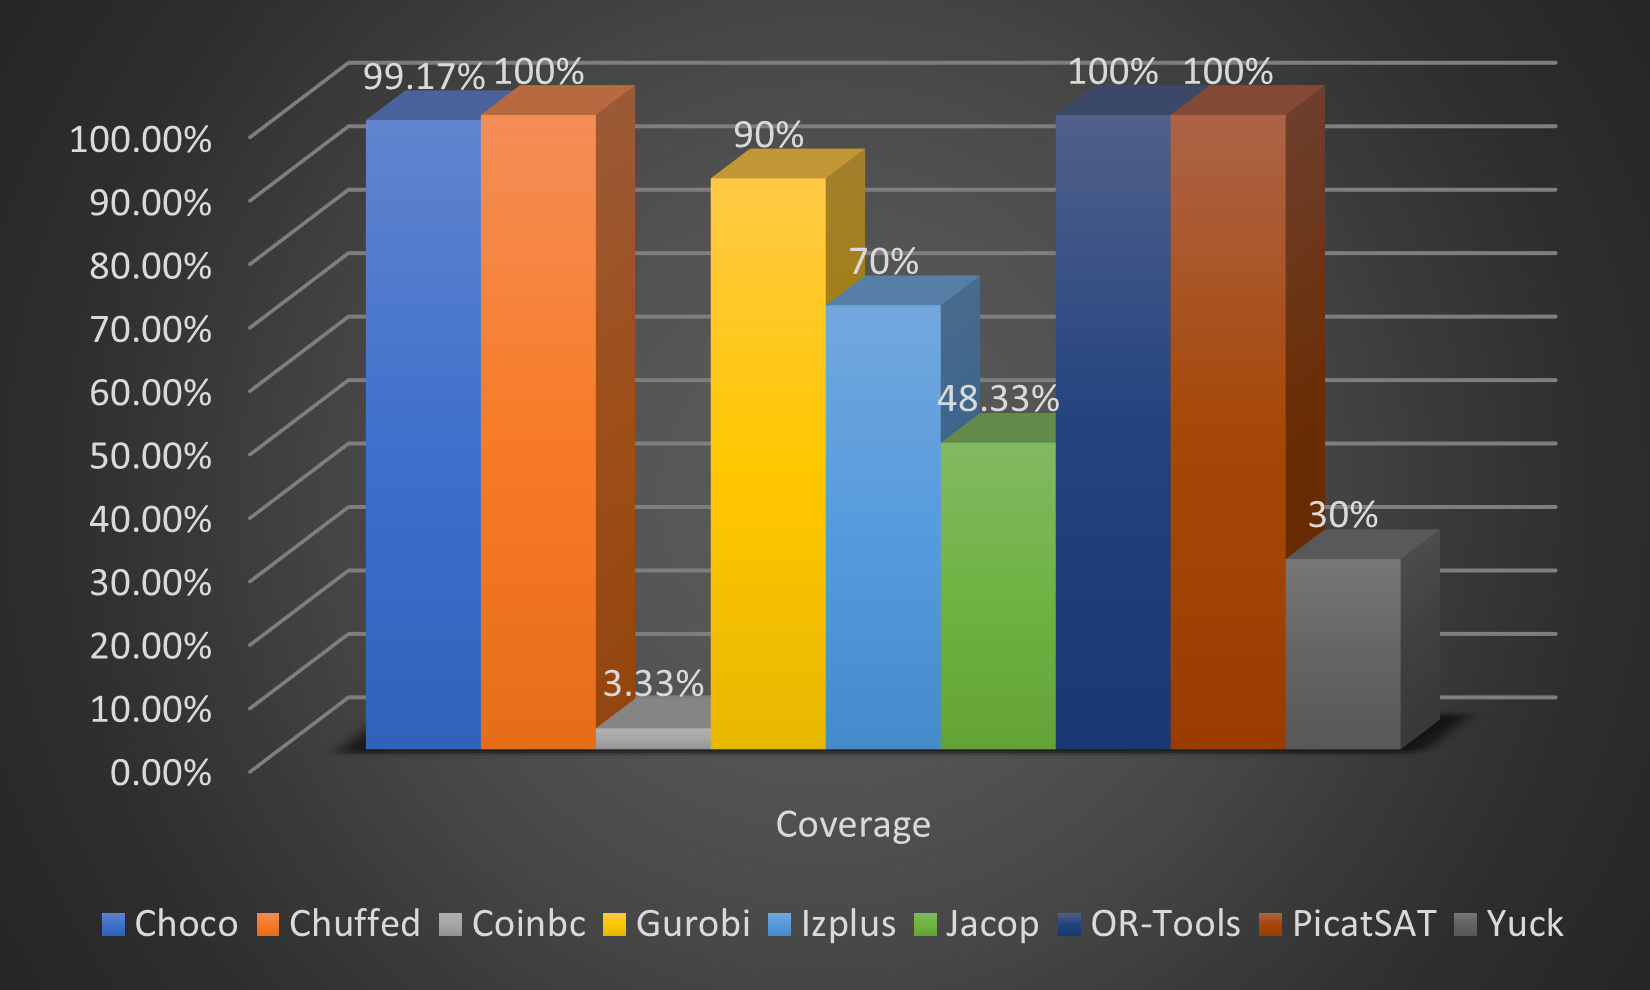
\includegraphics[width=0.6\textwidth]{figs/coverage.png}
    \caption{Overall coverage rates of each solver}
    \label{eva2}
\end{figure}
Table~\ref{tab:solvedcase} shows the solved problems for each solver. Based on the data in Table~\ref{tab:solvedcase},
Figure~\ref{eva2} shows the overall coverage rates for different solvers, which indicates that there are only 3 solvers' overall coverage rates are 100 percent.
In addition, Table~\ref{tab:solvedcaseforeach difficulty} separately shows the solved problems of different difficulties for each solver. Accordingly, Figure~\ref{fig:comparisonIQtwist} illustrates the change of coverage rates as the increasing of difficulty. It seems like the other solvers are not stable in different difficulties except there are 3 solvers which always keep 100 percent.
\begin{table}[htbp]
\centering
\caption{The solved cases for each difficulty}
\label{tab:solvedcaseforeach difficulty}
\begin{tabular}{|l|l|l|l|l|l|}
\hline
	    &Start&	Junior&	Expert&	Master&	Wizard\\
\hline
Choco   &23   &24 &24 &24 &24\\
\hline
Chuffed	&24   &24 &24 &24 &24\\
\hline
Coinbc	&4    &0  &0  &	0 &0\\
\hline
Gurobi	&24   &22 &20 &	23&19\\
\hline
Izplus	&23   &21 &13 &	17&10\\
\hline
Jacop	&20   &9  &11 &13 &5\\
\hline
Ortool	&24   &24 &24 &	24&24\\
\hline
PicatSAT&24   &24 &24 &24 &24\\
\hline
Yuck    &13	  &6  &2  &7  &8\\
\hline
\end{tabular}
\end{table}
\begin{figure}[H]
    \centering
    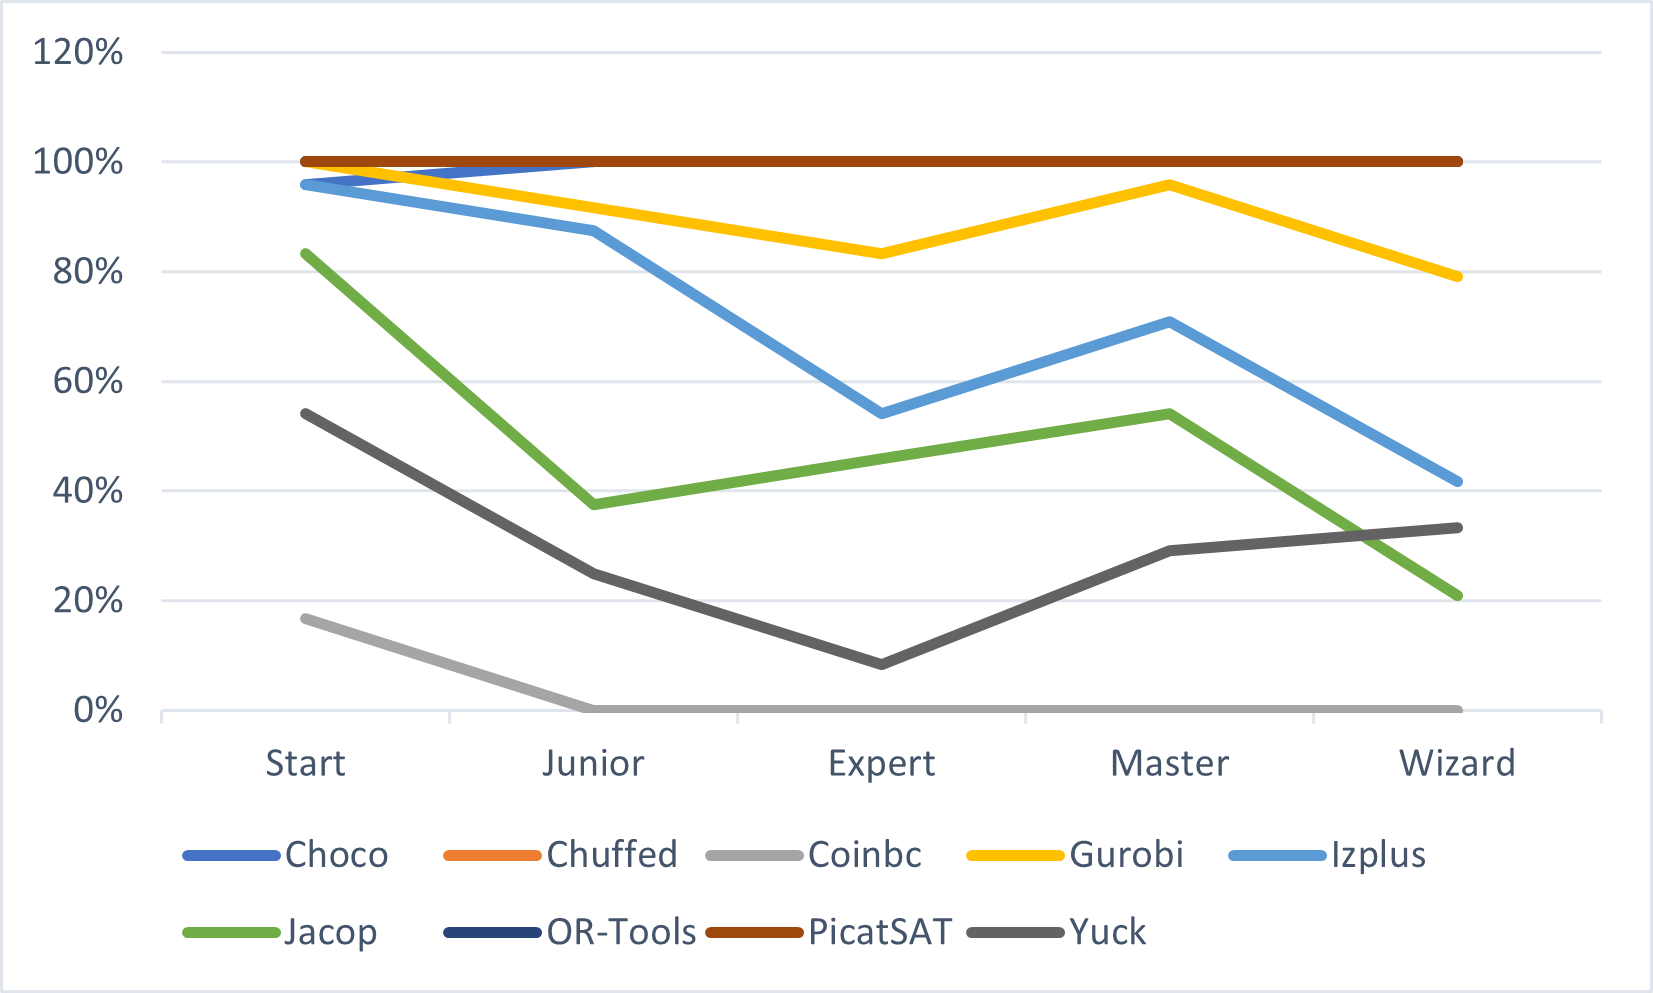
\includegraphics[width=0.6\textwidth]{figs/separated coverage.png}
    \caption{Coverage rates of each difficulty}
    \label{fig:comparisonIQtwist}
\end{figure}
Therefore, compared with other solvers, picatSAT, ortool and chuffed take advantage in coverage rates.
\\Secondly, all the execution times has been shown in Figure~\ref{fig:execution times}.
\begin{figure}[H]
    \centering
    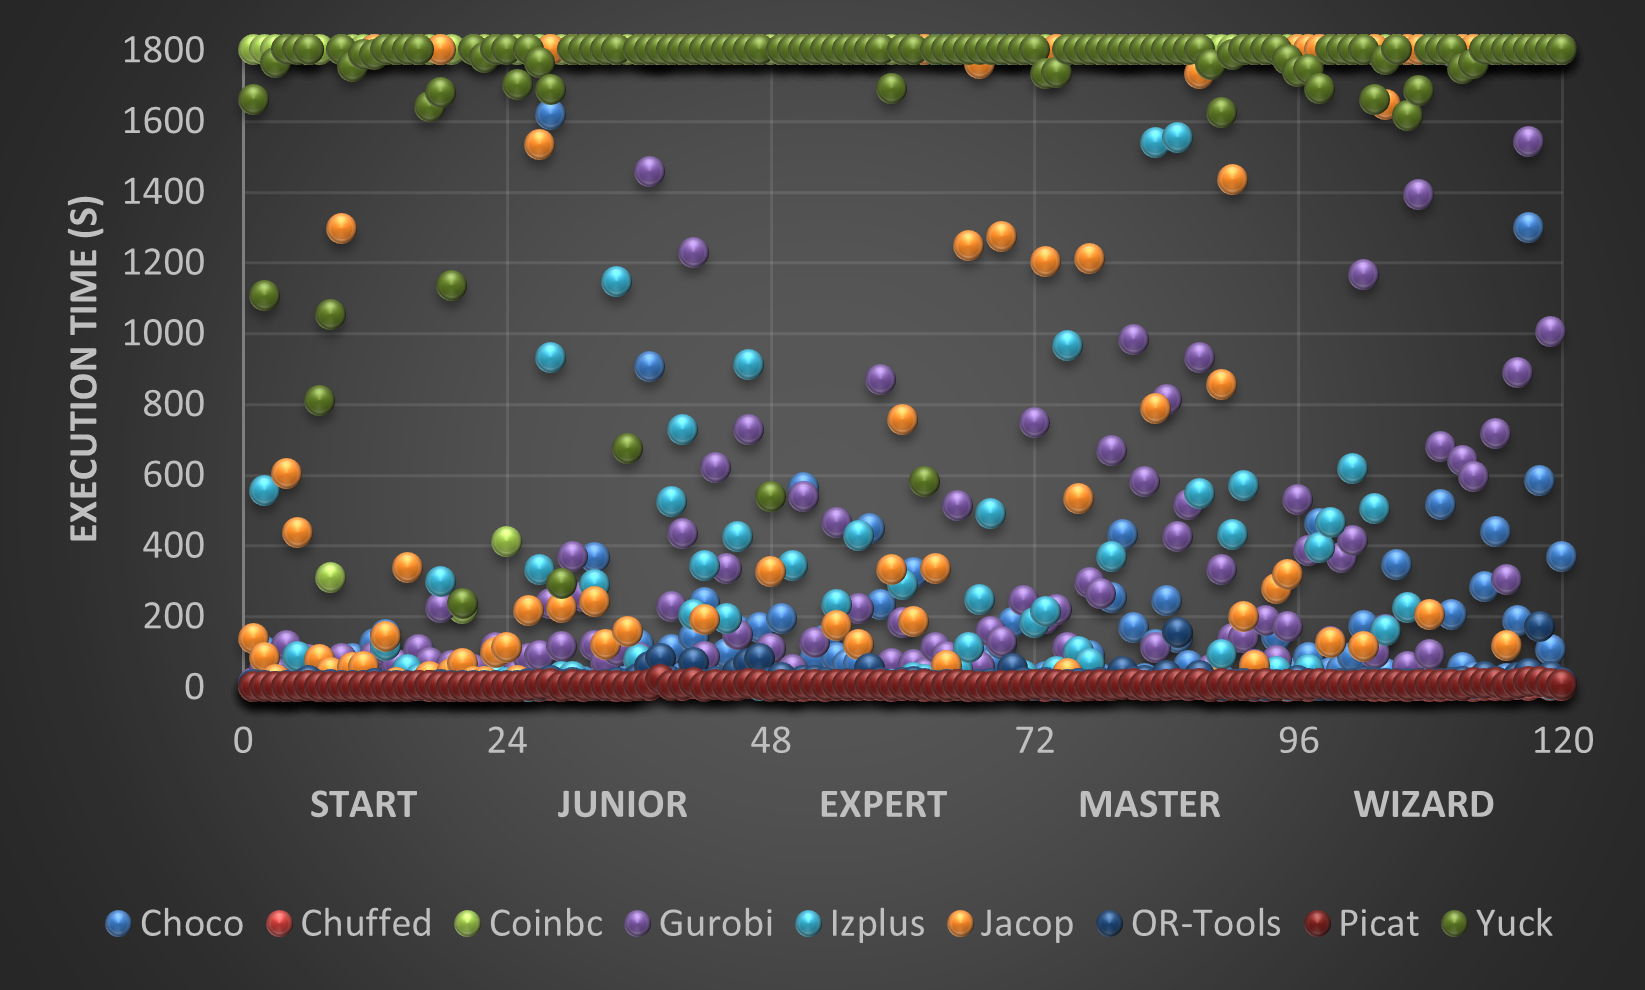
\includegraphics[width=0.6\textwidth]{figs/all_point_IQtwist.png}
    \caption{All execution times for all solvers}
    \label{fig:execution times}
\end{figure}
Figure~\ref{fig:execution times} indicates that chuffed, picatSAT and ortool takes huge advantages compared with other solvers because the three solvers can solve each problem in 200 seconds. More specifically, according to Figure~\ref{fig:3solvers1}, most of the execution times of chuffed and picatSAT are close, and they are usually better than ortool.
\begin{figure}[htbp]
\centering
\begin{subfigure}[b]{.48\textwidth}
\centering
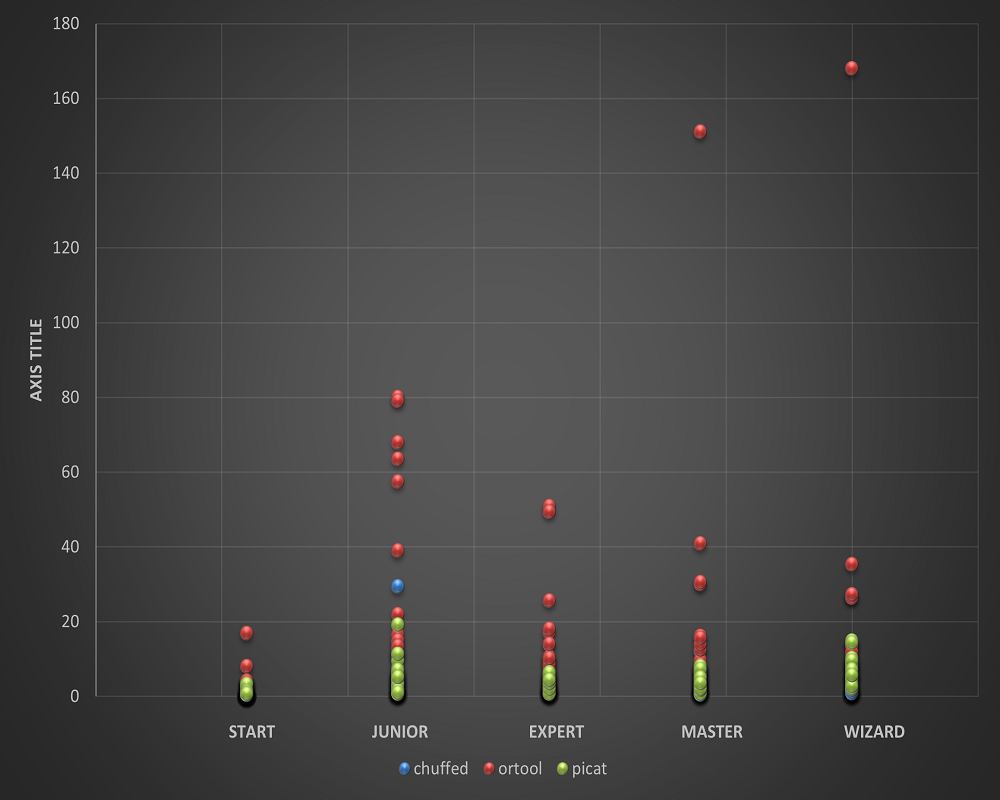
\includegraphics[width=\textwidth]{figs/threesolverpoints.png}
\caption{Execution times for chuffed, picatSAT and ortool}
\label{fig:3solvers1}
\end{subfigure}
\begin{subfigure}[b]{.48\textwidth}
\centering
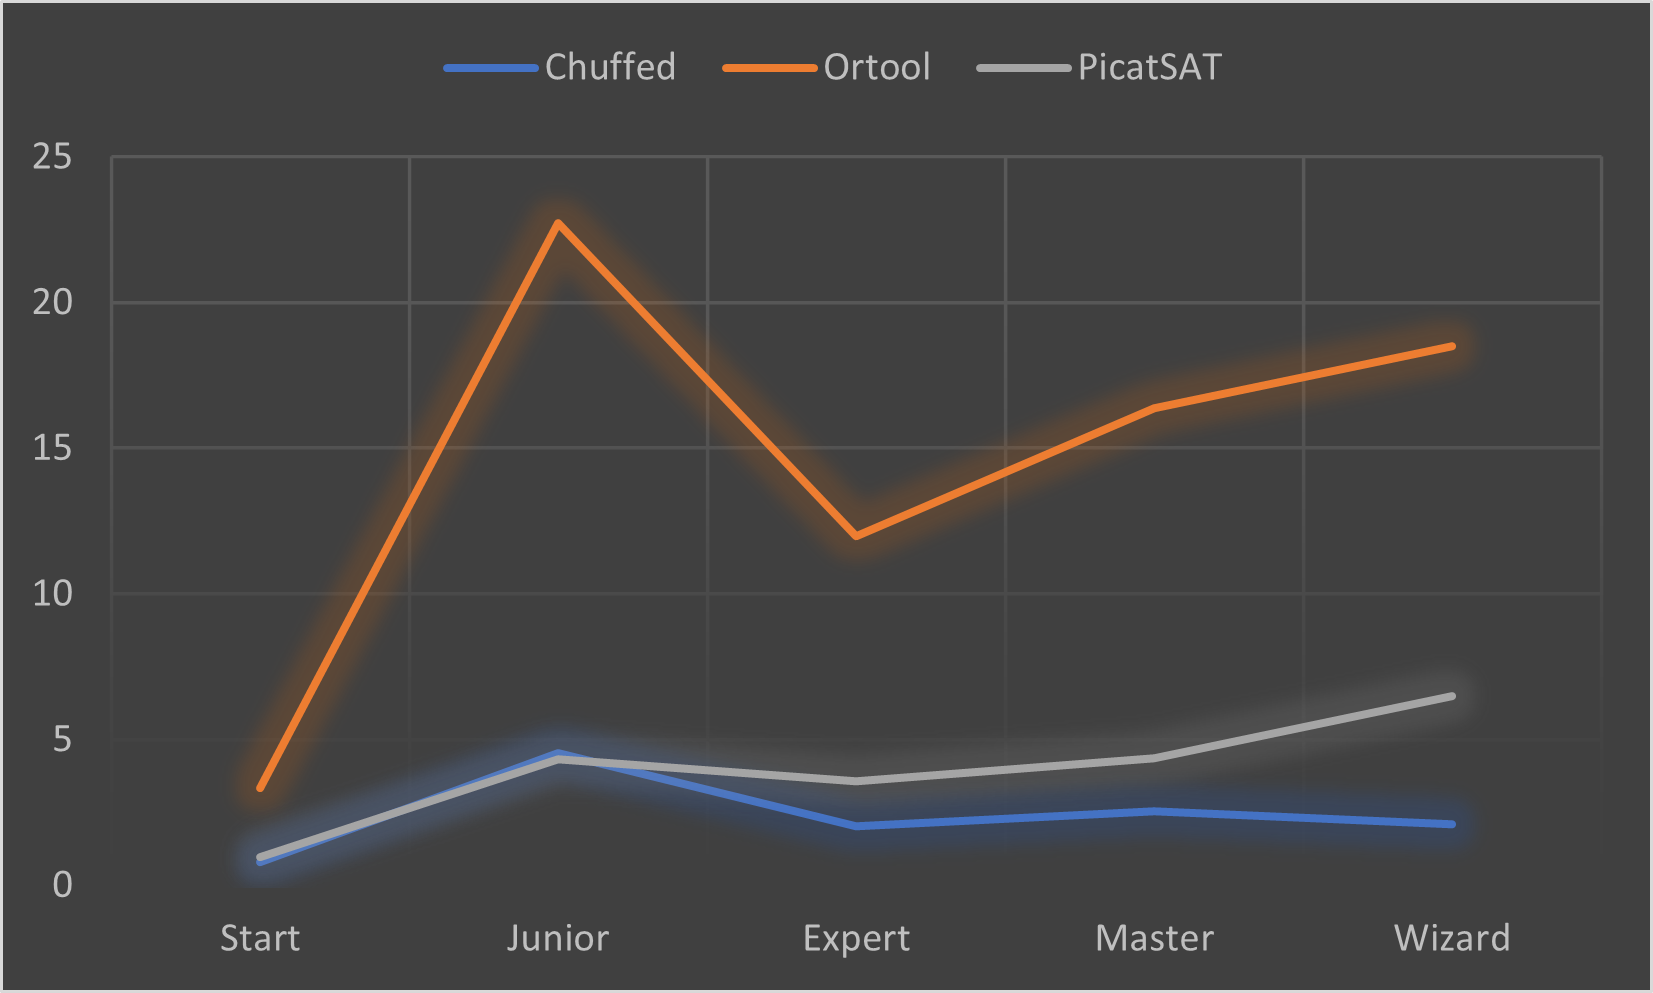
\includegraphics[width=\textwidth]{figs/Three comparison.png}
\caption{Average execution times for chuffed, picatSAT and ortool}
\label{fig:3comparison}
\end{subfigure}
\caption{The execution time comparisons between chuffed, picatSAT and ortool }
\label{fig:3comparisonsssss}
\end{figure}
Furthermore, Figure~\ref{fig:3comparison} indicates that the chuffed spends less time than picatSAT except in the "junior" difficulty.
\\In short, although all of chuffed, picatSAT and ortool can get the result for each problem in 30 minutes, the Chuffed possesses the best performance in IQ Twist.
\subsection{Zig Zag Puzzler Result}
\label{sec:Zig Zag Puzzlerresult}
In Zig Zag Puzzler booklet, there is a total of 80 problems, 40 of them belong to playing mode1, and the other 40 belong to playing mode2. For each playing mode, every 8 problems make up a difficulty. 
\subsubsection{Playing Mode1}
Firstly, for each solver, we can calculate the coverage rates by the Equation~\ref{equation:coverage}.
\begin{table}[htbp]
\centering
\caption{Overall solved problems for each solver in playing mode1}
\label{tab:solvedcase1}
\begin{tabular}{|l|l|l|l|l|l|l|l|l|}
\hline
Choco & Chuffed & Coinbc& Gurobi & Izplus&Jacop& Ortool& PicatSAT&Yuck \\
\hline
40   &40      & 20    & 35    &29     &33   &40    &40      &20\\
\hline
\end{tabular}
\end{table}
According to the data in Table~\ref{tab:solvedcase1}, Figure~\ref{fig:mode1eva2} indicates that there are 4 solvers keep 100 percent in the overall coverage.
\begin{figure}[H]
     \centering
    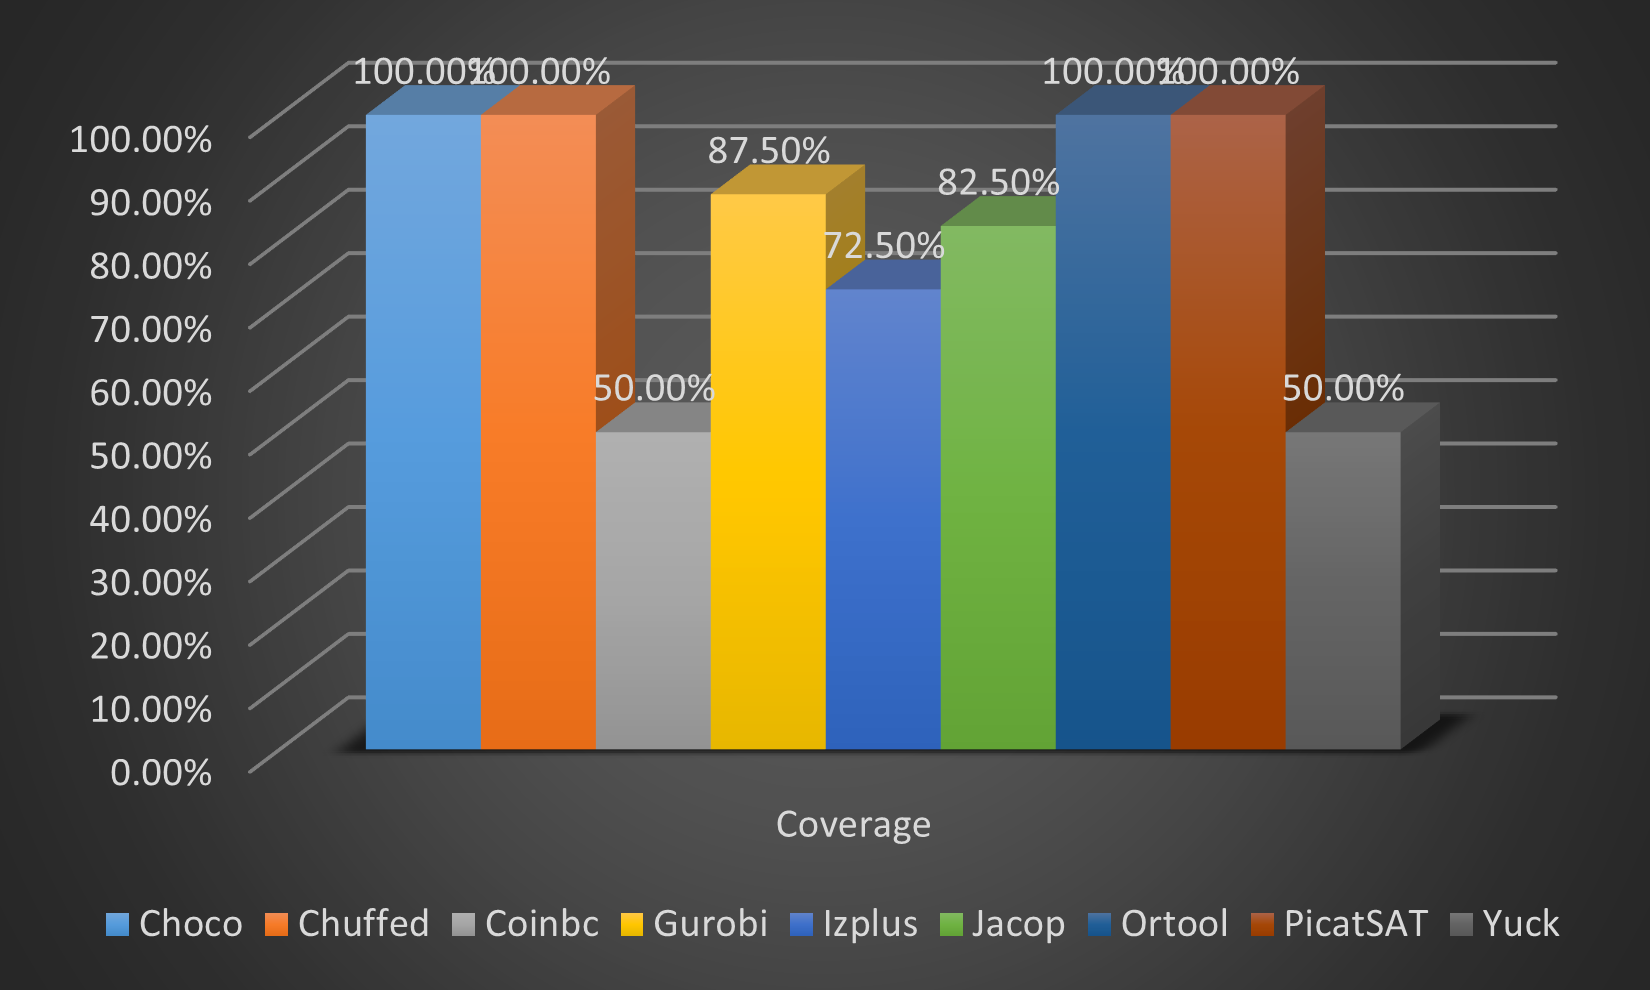
\includegraphics[width=0.6\textwidth]{figs/mode1coverage.png}
    \caption{Overall coverage rates of each solver}
    \label{fig:mode1eva2}
\end{figure}
\begin{table}[htbp]
\centering
\caption{The solved cases for each difficulty in playing mode1}
\label{tab:solvedcaseforeach difficulty1}
\begin{tabular}{|l|l|l|l|l|l|}
\hline
	    &Start	&Junior	&Expert	&Master	&Wizard\\
\hline
Choco	&8	&8	&8	&8	&8\\
\hline
Chuffed	&8	&8	&8	&8	&8\\
\hline
Coinbc	&8	&8	&4	&0	&0\\
\hline
Gurobi	&8	&8	&8	&8	&3\\
\hline
Izplus	&8	&8	&8	&4	&1\\
\hline
Jacop	&8	&8	&8	&5	&4\\
\hline
Ortool	&8	&8	&8	&8	&8\\
\hline
PicatSAT	&8	&8	&8	&8	&8\\
\hline
Yuck	&8	&8	&4	&0	&0\\
\hline
\end{tabular}
\end{table}
In addition, on account of Table~\ref{tab:solvedcaseforeach difficulty1}, Figure~\ref{fig:mode1eva4} reveals that the other 5 solvers' separated coverage is decreased as the difficulty increase. 
\begin{figure}[htbp]
    \centering
    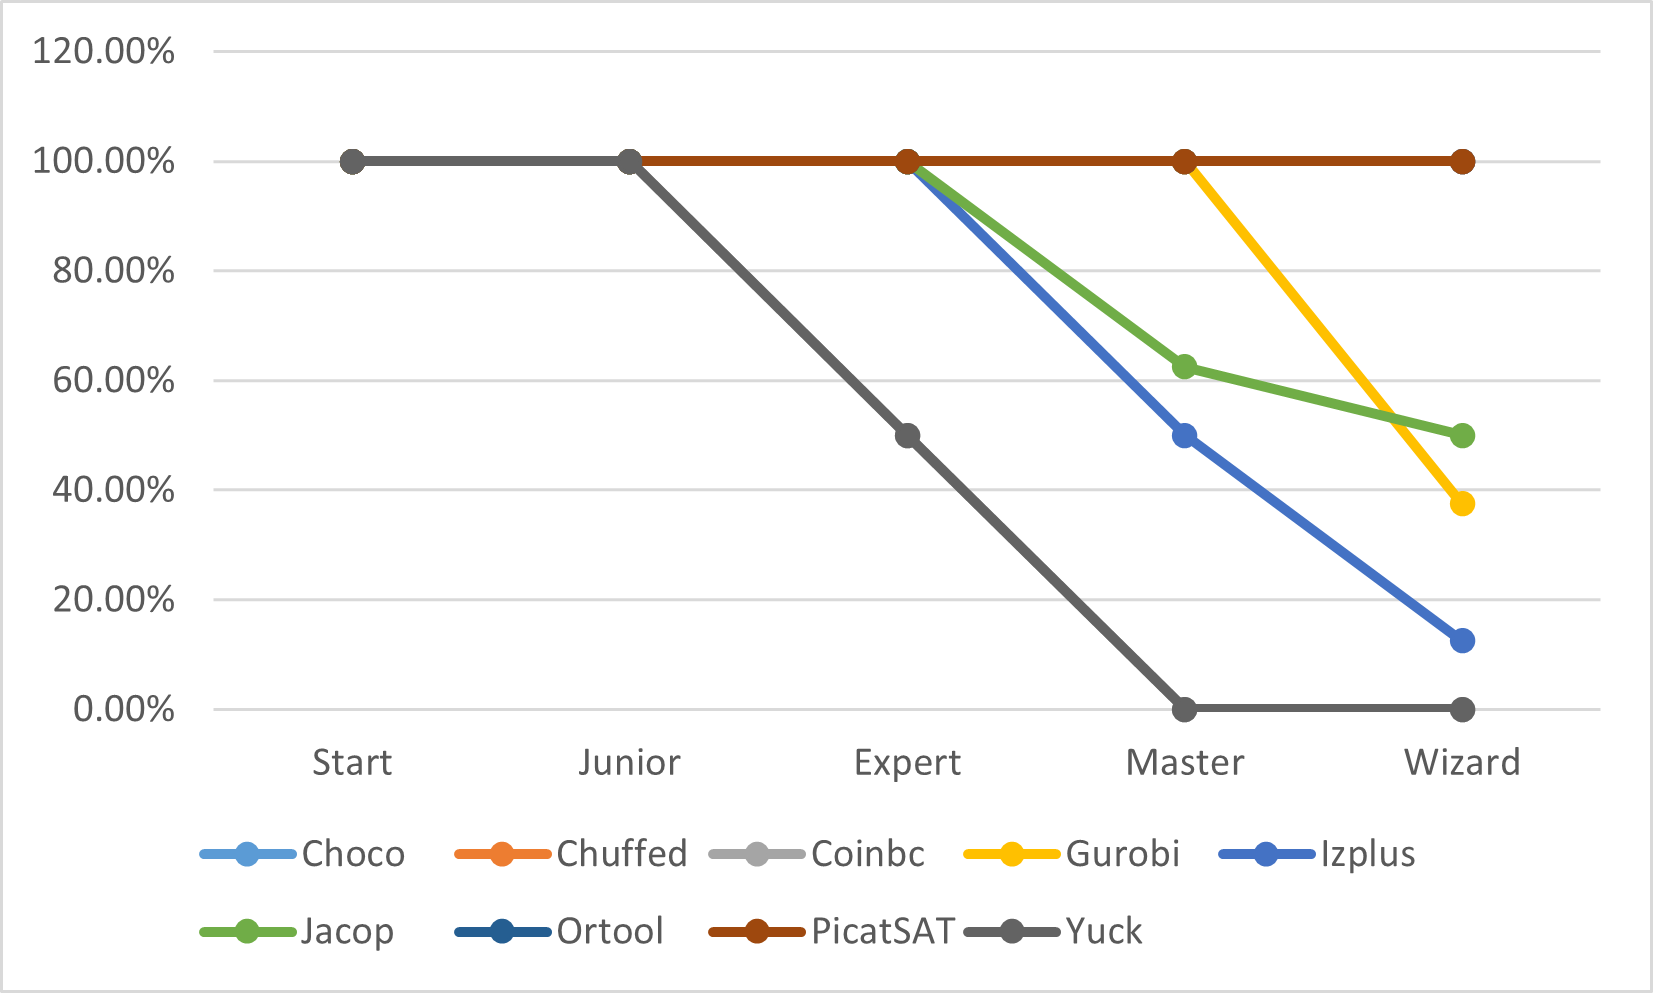
\includegraphics[width=0.6\textwidth]{figs/mode1seperatedcoverage.png}
    \caption{The coverage rates of each difficulty for each solver}
    \label{fig:mode1eva4}
\end{figure}
\\For execution times, Figure~\ref{fig:mode1time1} illustrates that except choco which spends a lot of time on some problems in  "wizard" difficulty, the other 3 solvers that contain 100 percent overall coverage rates only need very short time to solve each problem. 
\begin{figure}[htbp]
\centering
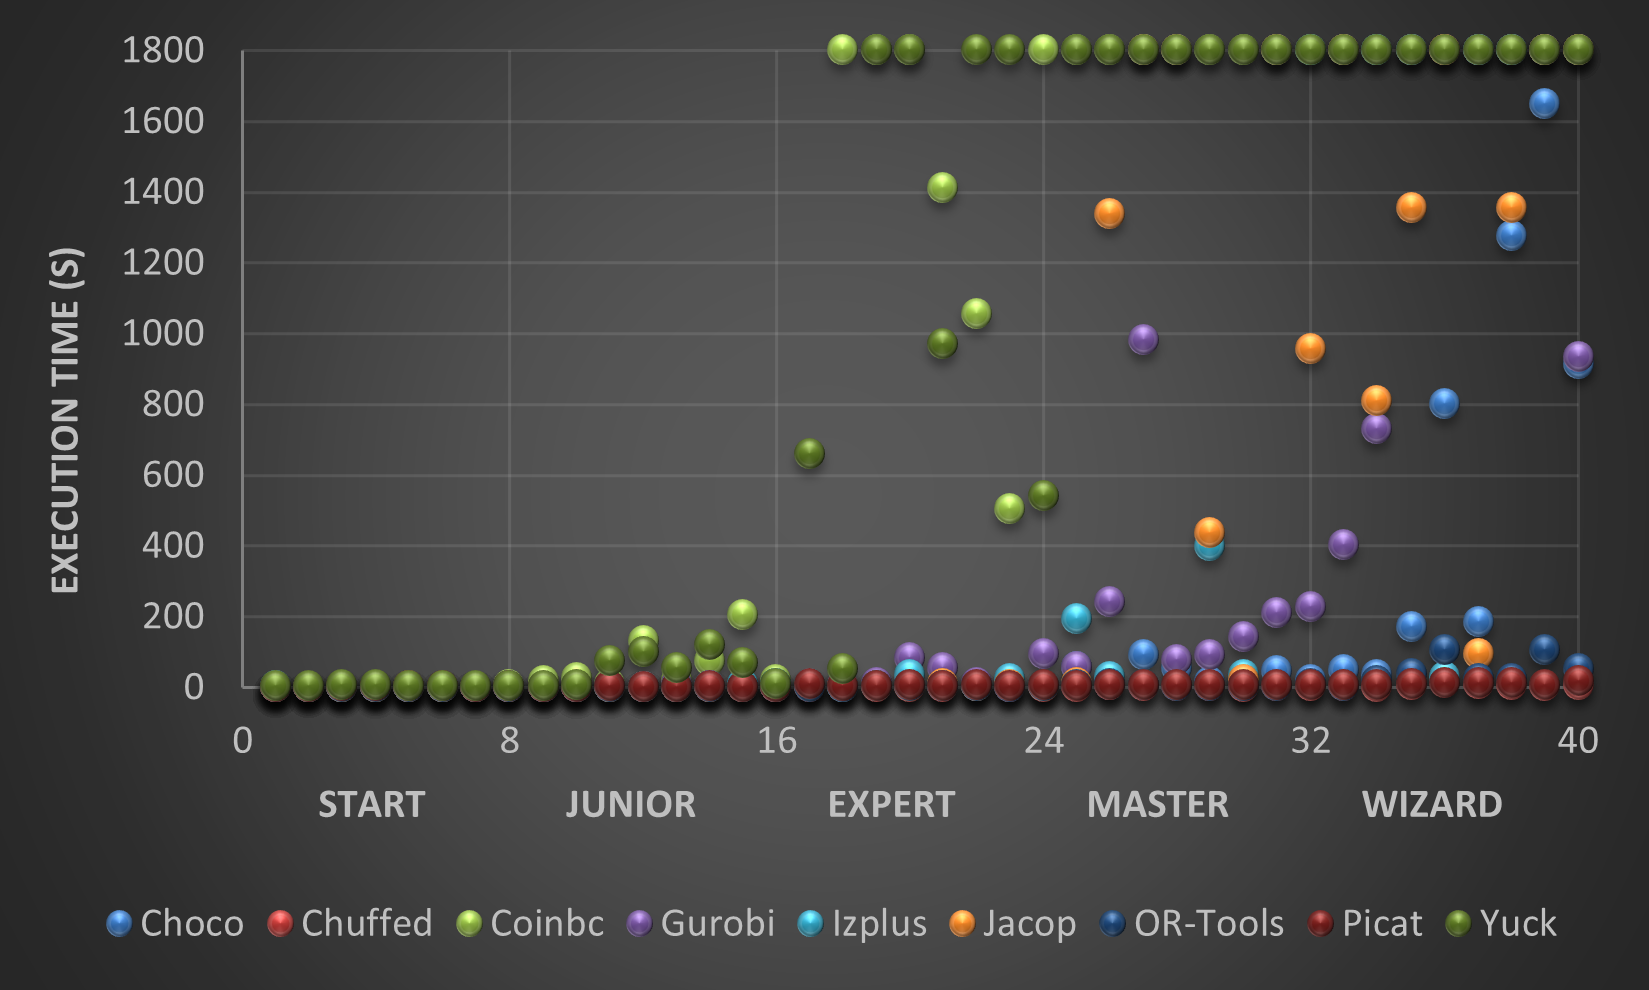
\includegraphics[width=0.6\textwidth]{figs/time1all.png}
\caption{Execution times for all problems}
\label{fig:mode1time1}
\end{figure}
Moreover, Figure~\ref{fig:time1three} reveals that for the problems in "wizard" difficulty, ortool and picatSAT spend more time for more cases. Accordingly, in Figure~\ref{fig:time1threeslope}, although the start point is very close, the growth rate of slopes for chuffed is much solver than ortool and picatSAT. Meanwhile, Figure~\ref{fig:mode1time1} reveals an obvious positive correlation between the execution time of different solvers and the difficulties. Therefore, chuffed has the optimal performance in execution time because of the lowest growth rate of slopes. 
\begin{figure}[htbp]
    \centering
    \begin{subfigure}[b]{0.48\textwidth}
     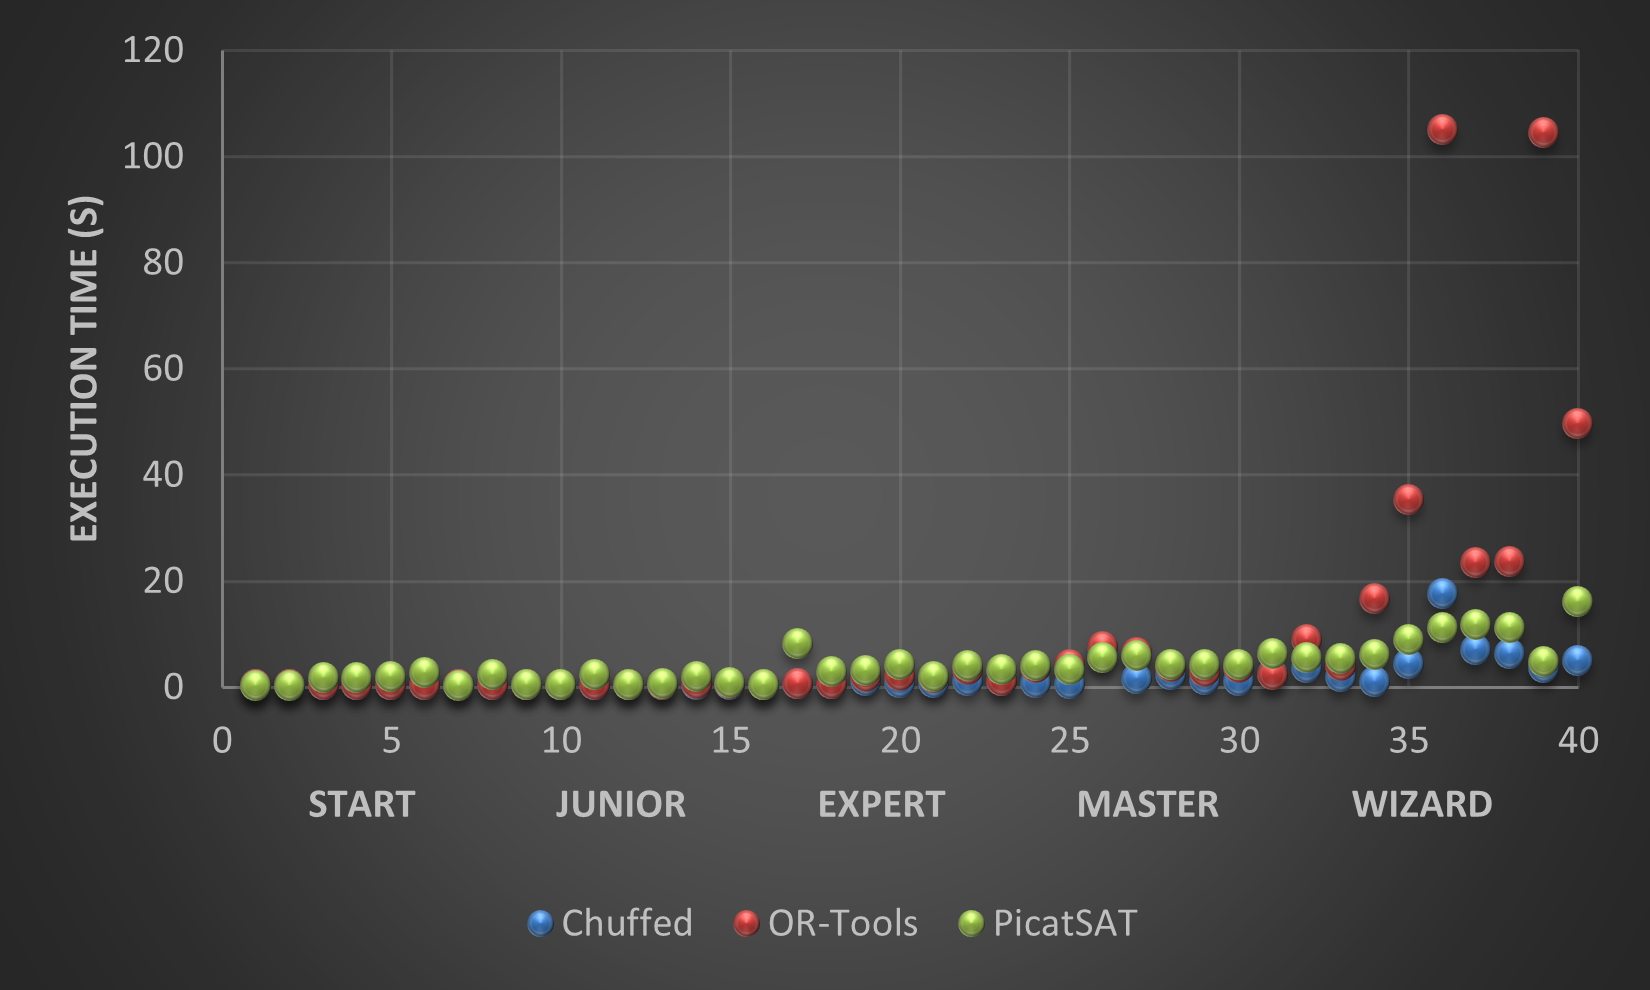
\includegraphics[width=\textwidth]{figs/time1three.png}
    \caption{Execution times for chuffed, picatSAT and ortool}
    \label{fig:time1three}
    \end{subfigure}
    \begin{subfigure}[b]{0.48\textwidth}
     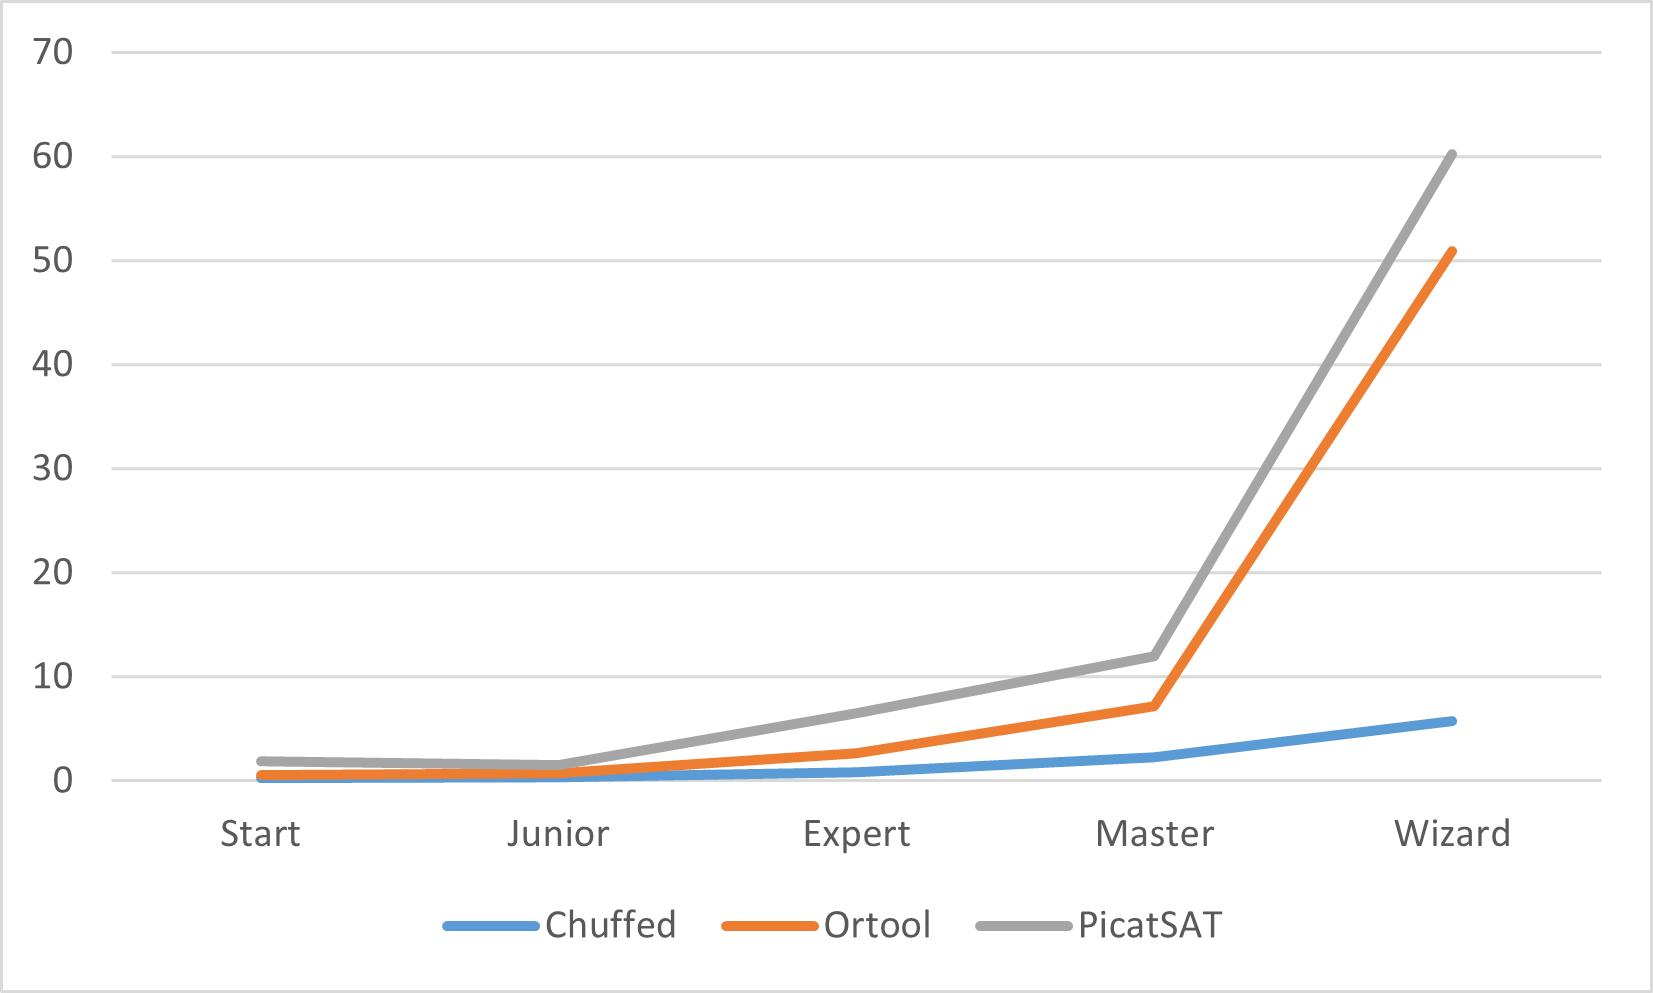
\includegraphics[width=\textwidth]{figs/mode1solverscomparison.png}
    \caption{Average execution time for chuffed, picatSAT and ortool}
    \label{fig:time1threeslope}
    \end{subfigure}
    \caption{The comparisons between chuffed, picatSAT and ortool}
\end{figure}
Overall, combine coverage and execution times, chuffed possess the best performance in Zig ZAG Puzzler playing mode1.
\subsubsection{Playing Mode2}
\begin{table}[htbp]
\centering
\caption{Overall solved problems for each solver in playing mode2}
\label{tab:solvedcase2}
\begin{tabular}{|l|l|l|l|l|l|l|l|l|}
\hline
Choco & Chuffed & Coinbc& Gurobi & Izplus&Jacop& Ortool& PicatSAT&Yuck \\
\hline
37   &40      & 12    & 34    &35     &32   &40    &40      &22\\
\hline
\end{tabular}
\end{table}
Based on Table~\ref{tab:solvedcase2}, as is shown in Figure~\ref{fig:mode2eva2}, the result of coverage rates is quite similar to the result of coverage rates in playing mode 1.
\begin{figure}[H]
     \centering
    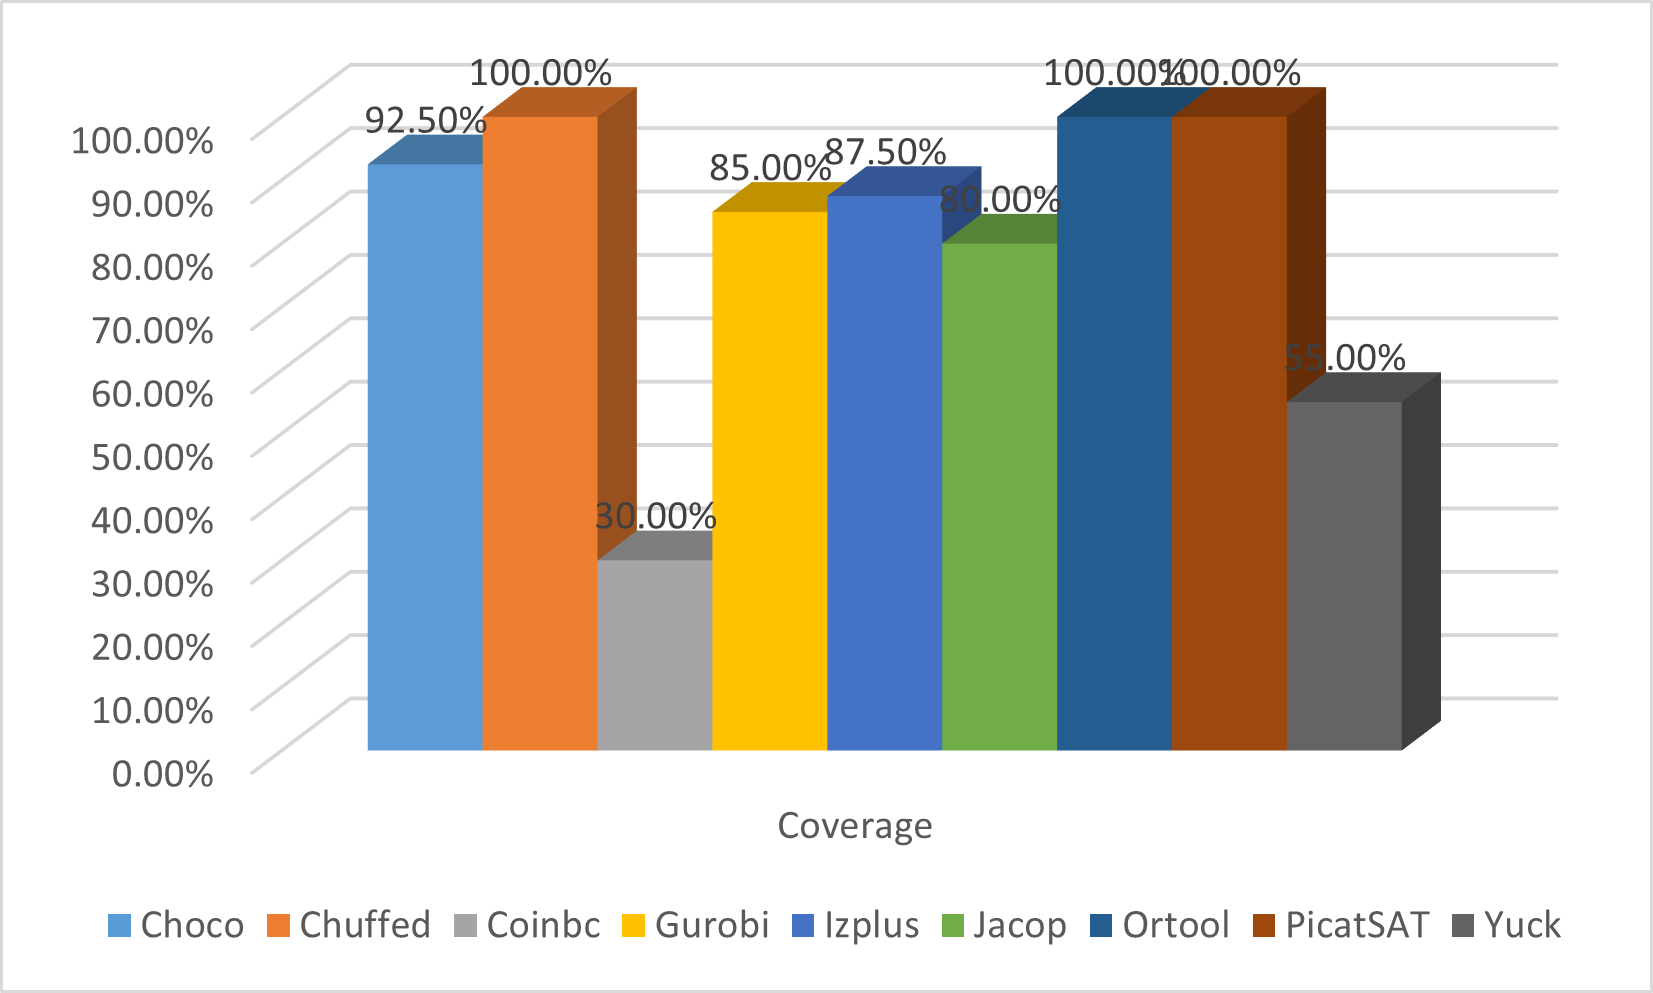
\includegraphics[width=0.6\textwidth]{figs/mode2coverage.png}
    \caption{Overall coverage rates of each solver}
    \label{fig:mode2eva2}
\end{figure}
Chuffed, picatSAT and ortool solve each problem in 30 minutes. 
\begin{table}[H]
\centering
\caption{The solved cases for each difficulty in playing mode2}
\label{tab:solvedcaseforeach difficulty2}
\begin{tabular}{|l|l|l|l|l|l|}
\hline
	    &Start	&Junior	&Expert	&Master	&Wizard\\
\hline
Choco	&8	&8	&8	&8	&5\\
\hline
Chuffed	&8	&8	&8	&8	&8\\
\hline
Coinbc	&7	&5	&0	&0	&0\\
\hline
Gurobi	&8	&8	&8	&7	&3\\
\hline
Izplus	&8	&8	&8	&7	&4\\
\hline
Jacop	&8	&8	&8	&7	&1\\
\hline
Ortool	&8	&8	&8	&8	&8\\
\hline
PicatSAT	&8	&8	&8	&8	&8\\
\hline
Yuck	&8	&8	&4	&2	&0\\
\hline
\end{tabular}
\end{table}
Meanwhile, according to the data in Table~\ref{tab:solvedcaseforeach difficulty2}, Figure~\ref{fig:mode2eva4} indicates that the other 6 solvers' separated coverage is decreased as the difficulty increase.
 \begin{figure}[H]
   \centering
    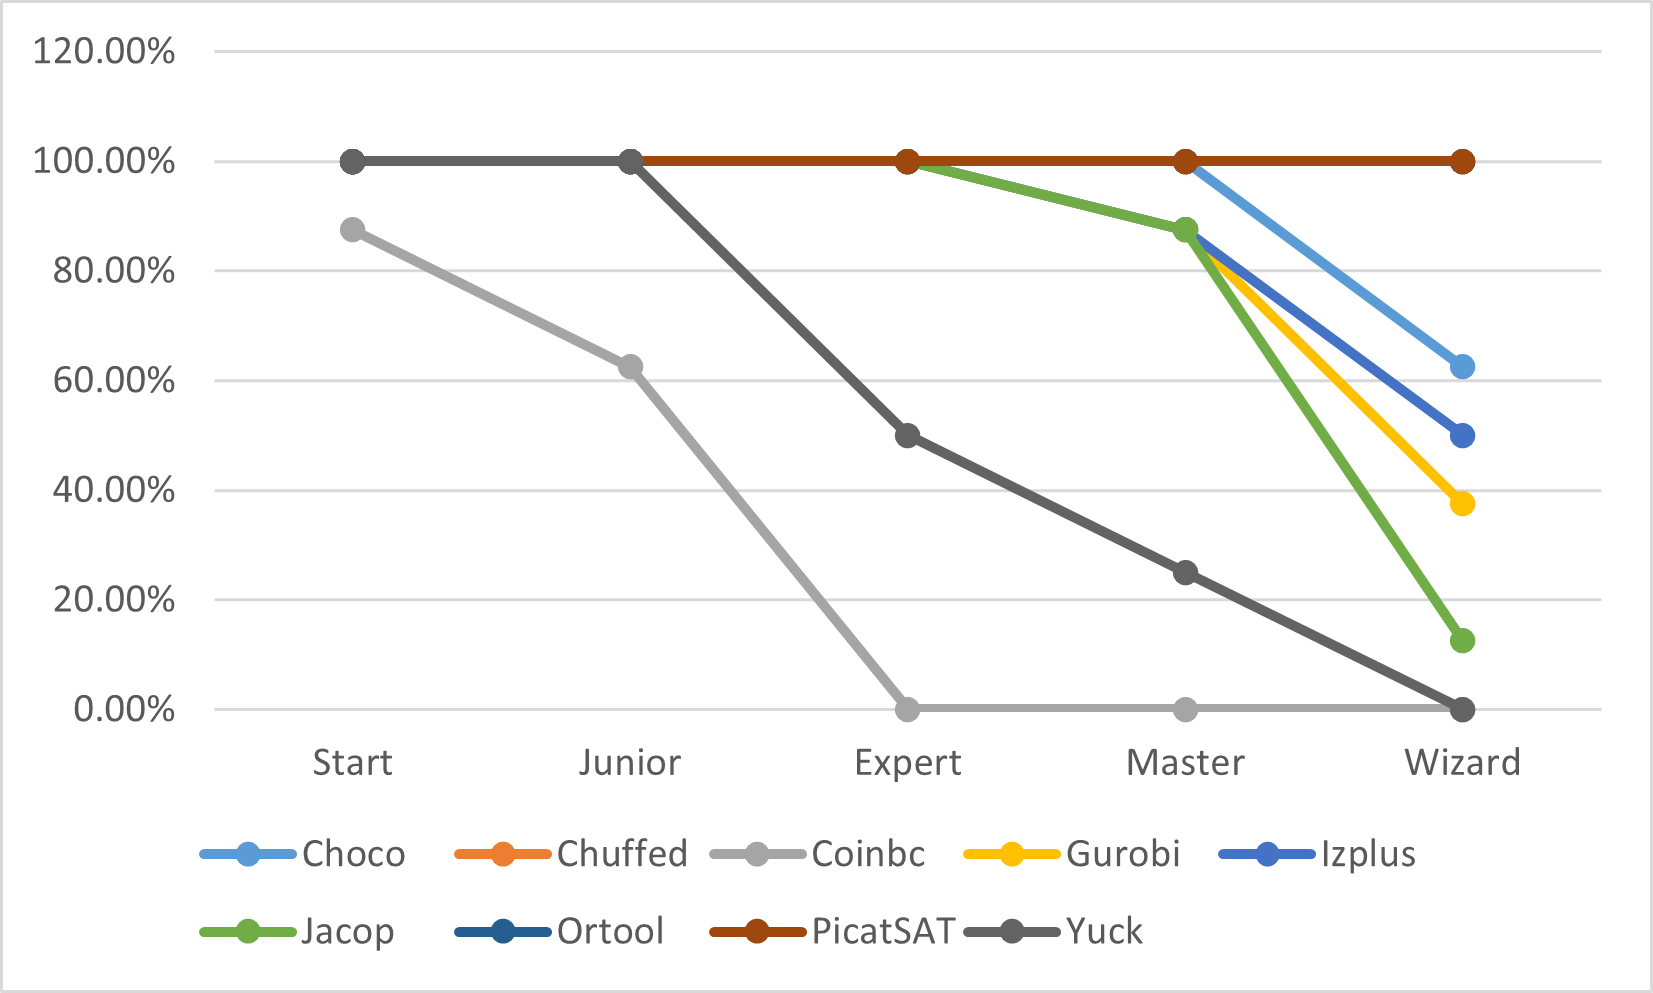
\includegraphics[width=0.6\textwidth]{figs/mode2seperatedcoverage.png}
    \caption{The coverage rates of each solver for different difficulties}
    \label{fig:mode2eva4}
\end{figure}
For the execution times, as is shown in Figure~\ref{fig:mode2time2}, almost all the solvers' execution times are a positive correlation with the difficulties. Again, chuffed, picatSAT and ortool spend less time to solve most problems. 
\begin{figure}[H]
    \centering
    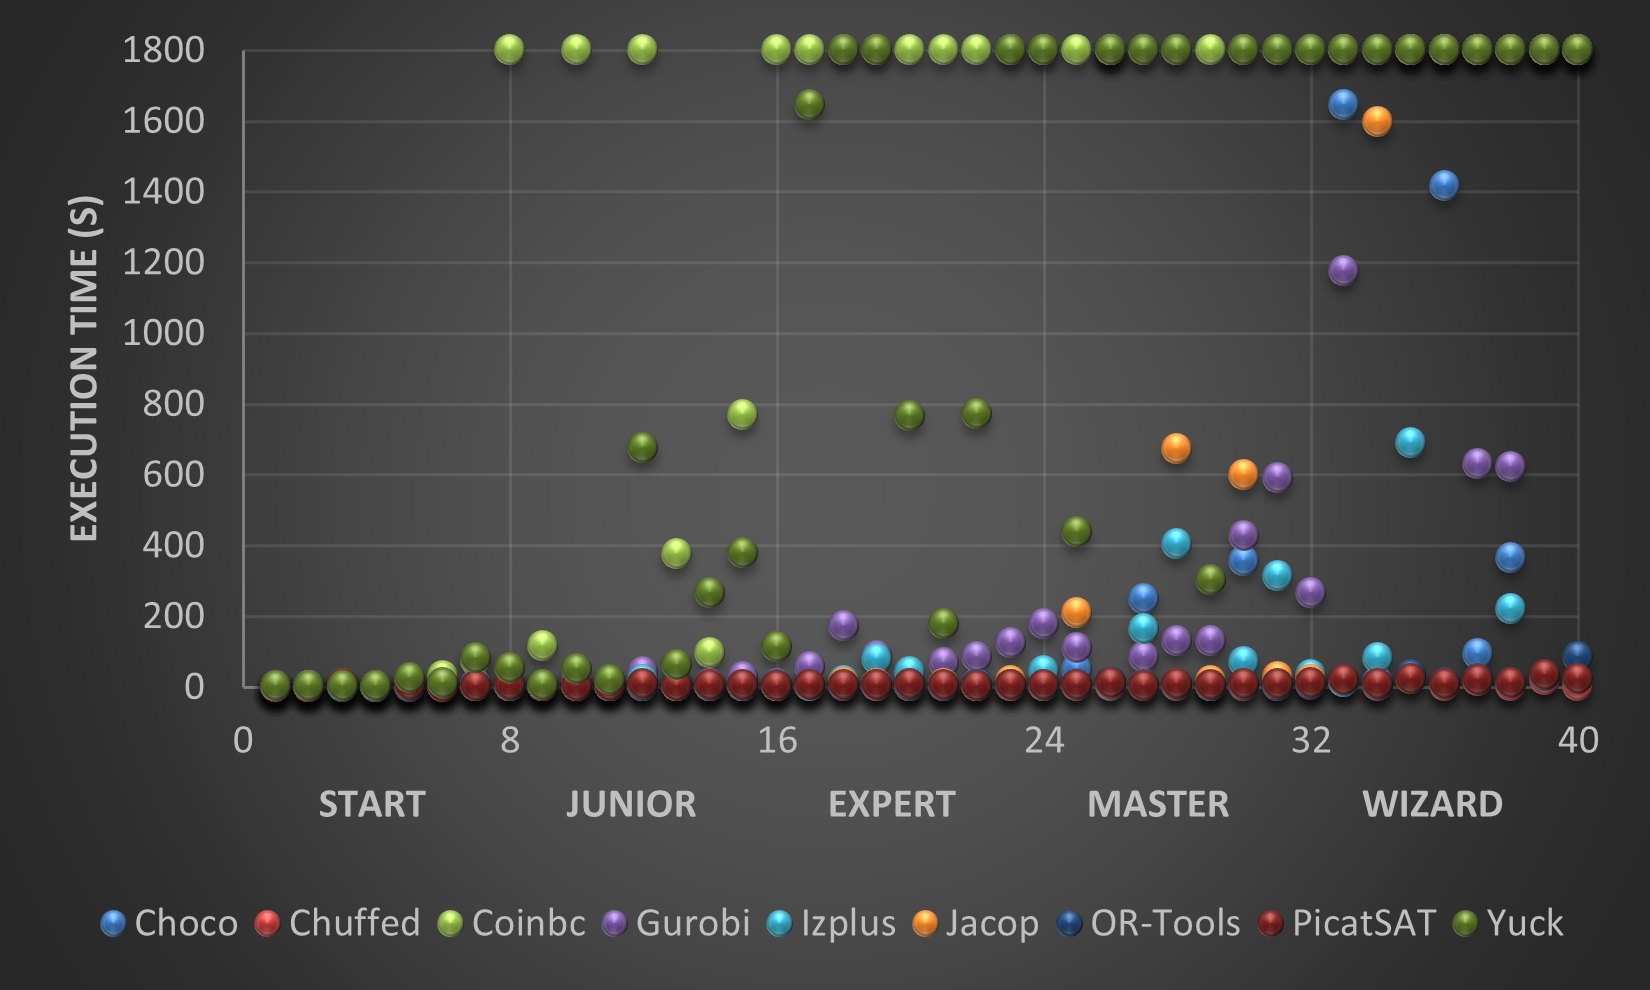
\includegraphics[width=0.6\textwidth]{figs/time2all.png}
    \caption{The execution times of solved problems}
    \label{fig:mode2time2}
\end{figure}
Similarly, on account of Figure~\ref{fig:comparisonlast}, chuffed achieves optimal performance. 
\begin{figure}[H]
\begin{subfigure}[b]{0.48\textwidth}
  \centering
    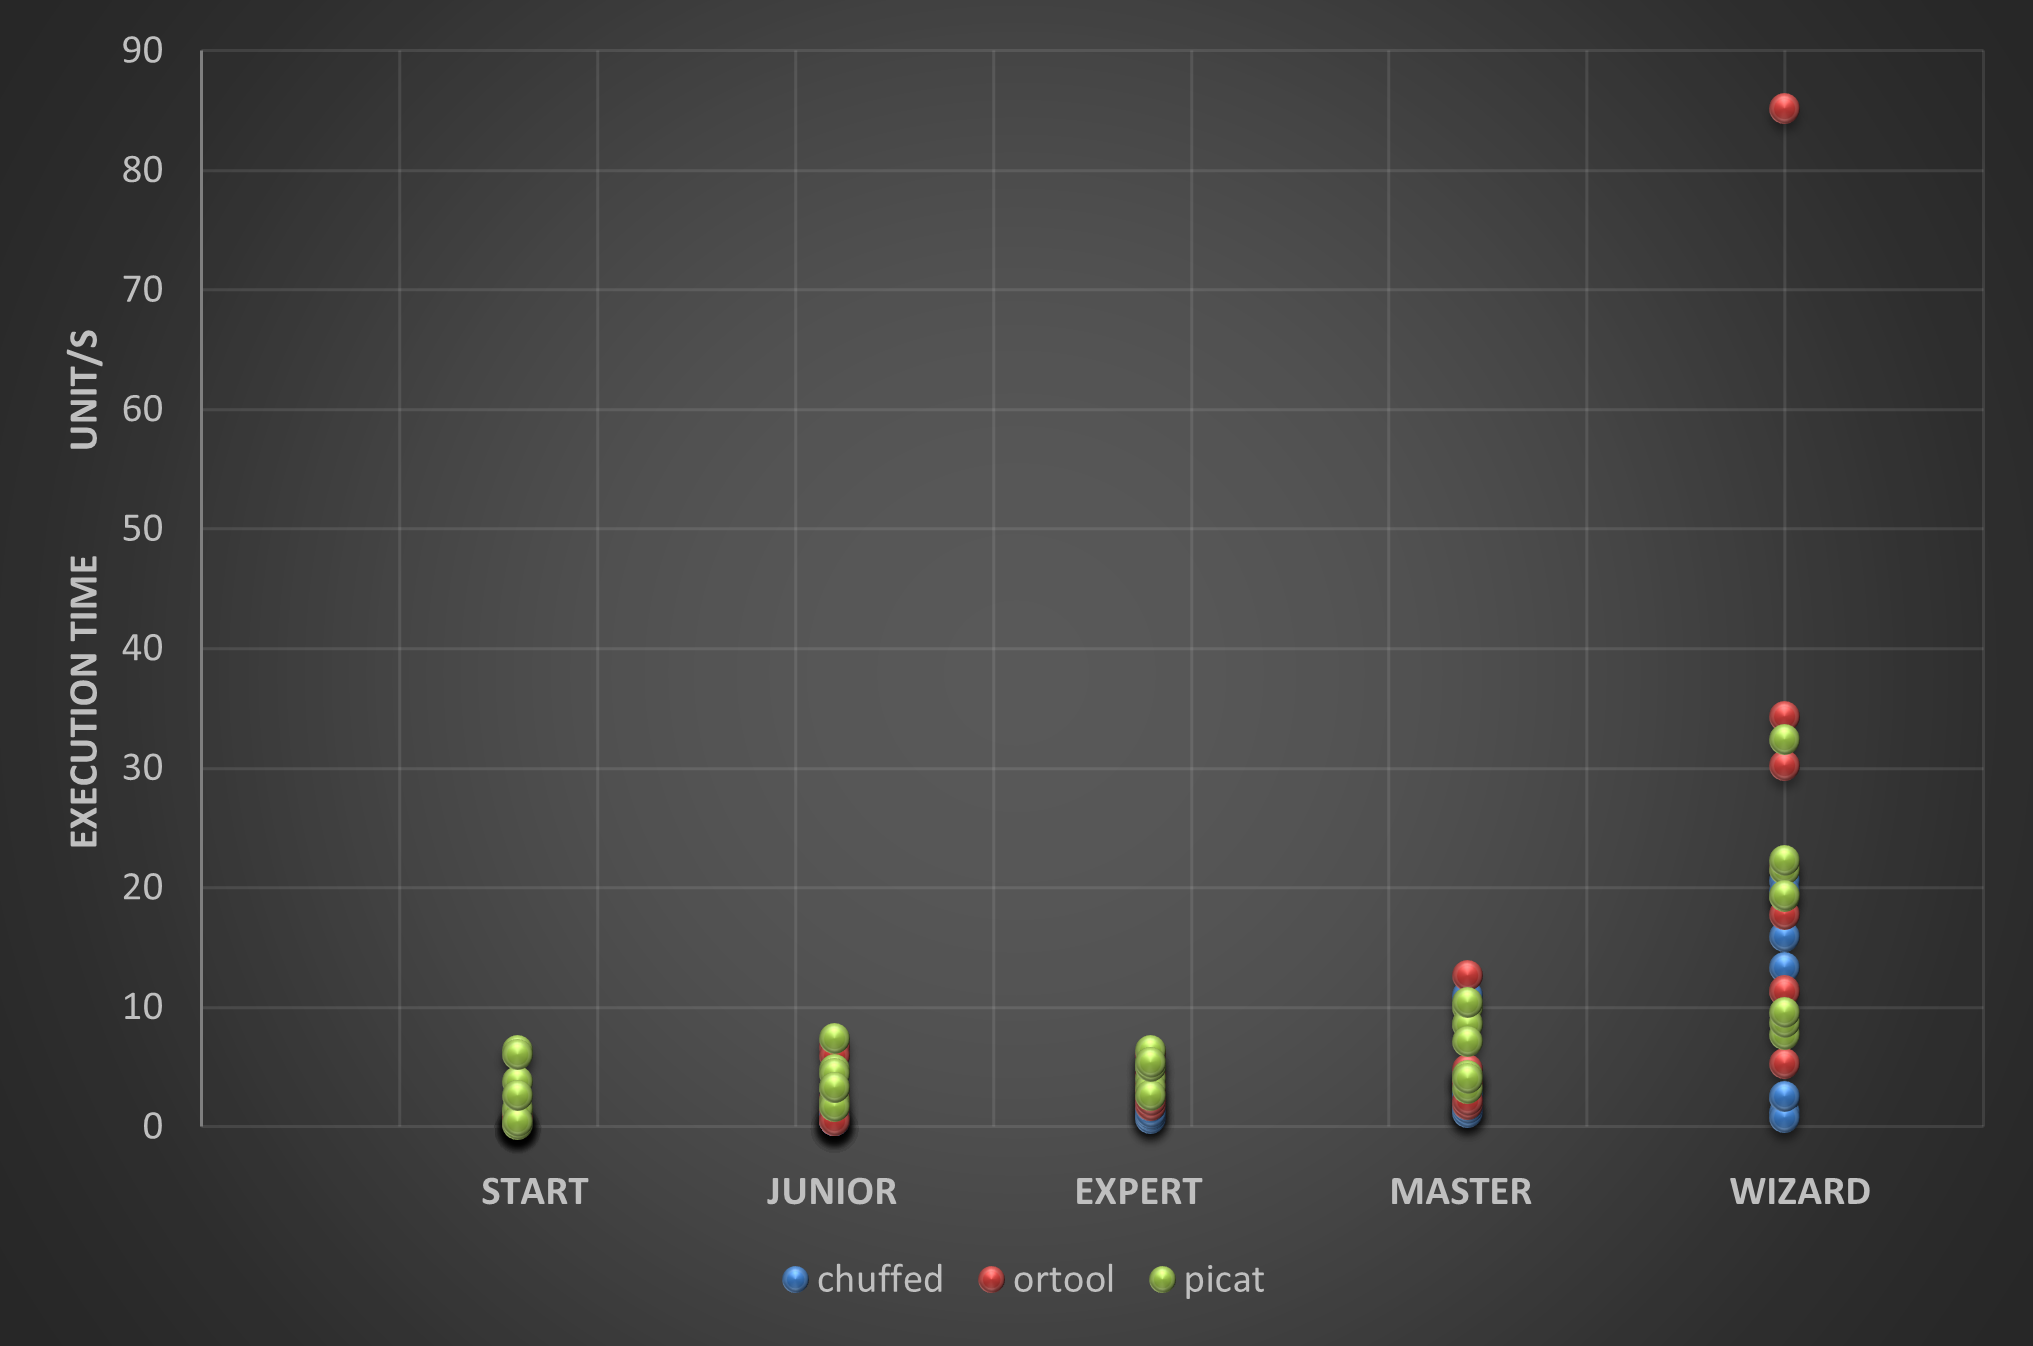
\includegraphics[width=\textwidth]{figs/time2three.png}
    \caption{Execution times for chuffed, picatSAT and ortool}
    \label{fig:compare}
\end{subfigure}
\begin{subfigure}[b]{0.48\textwidth}
 \centering
    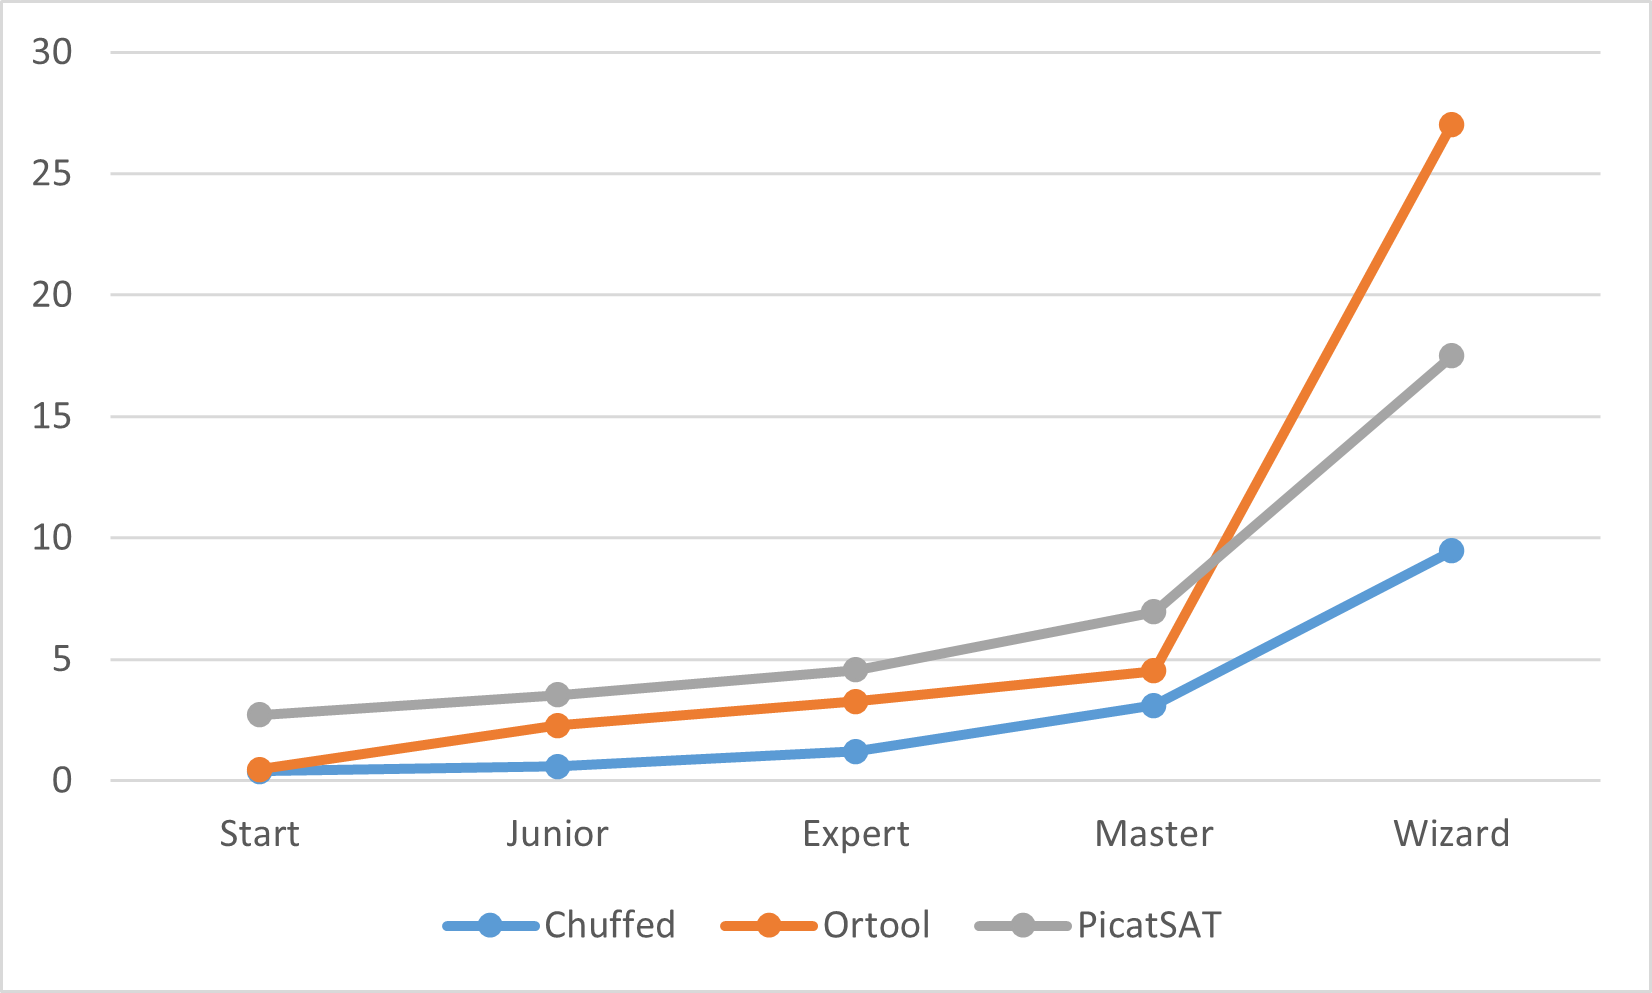
\includegraphics[width=\textwidth]{figs/Threecomparison2.png}
    \caption{Average execution times for chuffed, picatSAT and ortool}
    \label{fig:compare}
\end{subfigure}
\caption{Comparisons between  chuffed, picatSAT and ortool}
\label{fig:comparisonlast}
\end{figure}
\subsection{Summary}
\label{sec:Summary}
For all the problems in both IQ Twist and Zig Zag Puzzler, chuffed, picatSAT and ortool can solve each of them in 30 minutes. Meanwhile, their performances are more stable and the average execution times for each problem are only a few seconds. To sum up, compared with other solvers, chuffed, picatSAT and ortool have obvious advantage in such problems, moreover, the chuffed cost the shortest time in almost all problems. 
 